%%%%%%%%%%%%%%%%%%%%%%%%%%%%%%%%%%%%%%%%%
% "ModernCV" CV and Cover Letter
% LaTeX Template
% Version 1.1 (9/12/12)
%
% This template has been downloaded from:
% http://www.LaTeXTemplates.com
%
% Original author:
% Xavier Danaux (xdanaux@gmail.com)
%
% License:
% CC BY-NC-SA 3.0 (http://creativecommons.org/licenses/by-nc-sa/3.0/)
%
% Important note:
% This template requires the moderncv.cls and .sty files to be in the same 
% directory as this .tex file. These files provide the resume style and themes 
% used for structuring the document.
%
%%%%%%%%%%%%%%%%%%%%%%%%%%%%%%%%%%%%%%%%%

%----------------------------------------------------------------------------------------
%	PACKAGES AND OTHER DOCUMENT CONFIGURATIONS
%----------------------------------------------------------------------------------------

\documentclass[11pt,a4paper,sans]{moderncv} % Font sizes: 10, 11, or 12; paper sizes: a4paper, letterpaper, a5paper, legalpaper, executivepaper or landscape; font families: sans or roman
%\usepackage{footmisc}

\moderncvstyle{classic} % CV theme - options include: 'casual' (default), 'classic', 'oldstyle' and 'banking'
\moderncvcolor{blue} % CV color - options include: 'blue' (default), 'orange', 'green', 'red', 'purple', 'grey' and 'black'

\usepackage{natbib}
\usepackage[T1]{fontenc} %
\usepackage[utf8]{inputenc} % Packages de langue
\usepackage[greek,french]{babel} %
\usepackage{datetime}

\usepackage[top=1.5cm, bottom=1.5cm, left=1.5cm, right=1.5cm, scale=0.65]{geometry}	% Régler finement les marges

\usepackage{xcolor}												% Color box
%\usepackage[unicode=true,										%
%pdftex,pdfborder={0 0 0},										%
%bookmarks=true,bookmarksnumbered=false,bookmarksopen=false,	% Pretty links in pdf
%breaklinks=false,linkbordercolor=white,colorlinks=false,		%
%backref=false,frenchlinks]{hyperref}							%

%\hypersetup{pdftitle={CV Michaël Roynard 2016},pdfauthor={Michaël Roynard}}

\usepackage{lipsum} % Used for inserting dummy 'Lorem ipsum' text into the template

%\usepackage[scale=0.75]{geometry} % Reduce document margins
%\setlength{\hintscolumnwidth}{3cm} % Uncomment to change the width of the dates column
%\setlength{\makecvtitlenamewidth}{3cm} % For the 'classic' style, uncomment to adjust the width of the space allocated to your name

%----------------------------------------------------------------------------------------
%	NAME AND CONTACT INFORMATION SECTION
%----------------------------------------------------------------------------------------

\name{Michaël}{ROYNARD}

% All information in this block is optional, comment out any lines you don't need
\title{Chercheur postdoc au Laboratoire de Recherche de l'EPITA (LRE)}
\address{5 rue d'Effiat, Bât. 4, App. 201}{91380 Chilly-Mazarin}
\mobile{(+33) 6 44 24 65 76}
%\phone{(000) 111 1112}
%\fax{(000) 111 1113}
\email{michaelroynard@gmail.com}
%\email{michael.roynard@epita.fr}
\homepage{dutiona.github.io}
\extrainfo{\href{https://github.com/dutiona/}{Profil Github}}
%\photo[70pt][0.4pt]{picture} % The first bracket is the picture height, the second is the thickness of the frame around the picture (0pt for no frame)
\quote{Programmation générique en C++ moderne pour le traitement d'images}

%----------------------------------------------------------------------------------------

\begin{document}

\makecvtitle % Print the CV title

%----------------------------------------------------------------------------------------
%	WORK EXPERIENCE SECTION
%----------------------------------------------------------------------------------------

\section{Expérience professionnelle}

%\subsection{Vocational}
\cventry{2017--Présent}
{Doctorant}
{LDE, EPITA}
{Le Kremlin-Bicêtre}
{}
{Intégration de l’équipe Image du LRE (anciennement LRDE) pour travailler, durant ma thèse, sur le projet \href{https://www.lre.epita.fr/wiki/Olena}{Olena} (Pylene). \'Etude des possibilités offertes par les nouvelles normes du langage C++, notamment en terme de généricité, pour améliorer la bibliothèque Olena qui a été écrite au début des années 2000.
	\begin{itemize}
		\item Recherche sur la taxonomie des différents types d'image ainsi que les différents canvas d'algorithmes.
		\item Design et implémentation des concepts relatifs au traitement d'images.
		\item Publications : An Image Processing Library in Modern C++: Getting Simplicity and Efficiency with Generic Programming in Reproducible Research in Pattern Recognition~\cite{roynard.2019.rrpr}.
		\item Recherche sur l'utilisation des vues pour le traitement d'images dans le but de relever le niveau d'abstraction à l'image (et non au pixel) pour une design d'application plus optimum~\cite{roynard.2022.gpce}.
		\item Recherche sur les ponts depuis Python pour pouvoir utiliser la bibliothèque C++ depuis un script Python (par exemple images NumPy, deeplearning, ...), avec pybind11.
		\item Méthodologie agile, utilisation d'outils DevOps pour CI/CD: CMake, Gitlab-ci, Conan, Docker, Artifactory, etc.
		\item Expérience d'enseignement (C++, Théorie des langages rationnels, Base de données, Algorithmie).
	\end{itemize}
}


\cventry{2016--2017}
{Développeur C++ frontoffice (produit financier)}
{Murex SAS}
{Paris 16\up{ème}}
{1 an et 5 mois}
{Développeur au sein de l'équipe dédiée aux produits financiers relatifs aux changes de monnaies. Développement en C++/Python/Groovy de logique métier relative au marché financier et d'outils permettant d'améliorer la productivité au quotidien. Membre du collectif d'experts C++ de la société.
	\begin{itemize}
		\item Écriture d'outils d'intégration continue :
		      \begin{itemize}
			      \item Analyse statique du code et refactoring automatisé avec Clang.
			      \item Écriture et mise en place du serveur d'intégration continue Jenkins, écriture de pipelines spécifiques au workflow de notre équipe.
			      \item Utilisation avancée d'outils de gestion de versions : git (intégrée à Atlassian Stash) et Perforce. Branchement de ces outils sur Jenkins dans le workflow de l'équipe.
			      \item Sensibilisation aux problématiques liées au système de build et de packaging.
		      \end{itemize}
		\item Conception et design des nouvelles API (Application Programming Interface) ainsi que leur refonte des anciennes dans le but d'appliquer au maximum les principes SOLID et la loi de Déméter.
		\item Développement et débuggage de nombreuses fonctionnalités sur une base de code legacy très conséquente.
		\item Utilisation de techniques de refactoring en vue de rendre le code testable unitairement et d'inverser les dépendances pour extraire des fonctionnalités derrière des interfaces.
		\item Écriture de tests unitaires (gtest) et de tests d'intégration (fitnesse).
		\item Membre de la \og community of practice \fg nommée CppChapter dans le but de promouvoir le C++ moderne au sein des développeurs de la société (veille technologique permanente, organisation de conférences internes et externes : hébergement de Meetup liées au C++).
		\item Sensibilisation à la cross compilation avec gcc, msvc, solaris cc et clang sur linux, windows et solaris (sparc) ainsi qu'à leur support \og maison \fg ~des nouvelles normes.
	\end{itemize}}

%------------------------------------------------

\cventry{2015--2016}
{Développeur backend C++ en soutien à la simulation}
{CEA - Commissariat à l'Energie Atomique et aux Energies Alternatives}
{Saclay}
{9 mois}
{Développeur multitâches au sein du DRT/LIST/DISC/LDI (Laboratoire de Développement Informatique) sur le logiciel de contrôle non destructif CIVA.
	Développement en C++/Java/Python avec OpenCascade/VTK/ODE d'outils de modélisation mathématique (maths3D, moteurs physiques, simulations, ...) :
	\begin{itemize}
		\item Implémentation de nouvelles fonctionnalités
		\item Réalisation d'un visualisateur 3D en VTK.
		\item Optimisation de performance (algorithme de maillage de pièces CAO et mise en place de cache).
		\item Rédaction d'une documentation développeur.
		\item Débuggage du logiciel en vue d'une sortie de version majeure.
		\item Travail dans un laboratoire informatique moderne et dynamique.
	\end{itemize}}

%------------------------------------------------

\cventry{2014--2015}
{Développeur stagiaire}
{CEA - Commissariat à l'énergie atomique et aux énergies alternatives}
{Saclays}
{6 mois}
{Développement d’un module pour le logiciel CIVA permettant l’atterrissage d’un capteur sur une pièce à tester en prenant en compte les collisions et l’encombrement en utilisant un moteur physique :
	\begin{itemize}
		\item \'{E}tat de l’art sur les moteurs physiques existants
		\item Réalisation d’un benchmark pour déterminer quel moteur physique utiliser (et la faisabilité du problème avec ceux-ci).
		\item Mise au point et implémentation de l’algorithme en C++11 sous Visual studio 2013.
		\item Tests de performance et mise en forme sous une API
		\item Intégration dans CIVA
		\item Rédaction d’une documentation développeur
	\end{itemize}}

%------------------------------------------------

%\cventry{2012}
%{Développeur stagiaire}
%{THALES AVIONICS ELECTRICAL SYSTEMS SAS}
%{Région de Toulouse, France}
%{5 mois}
%{Développement d’un logiciel client lourd JAVA pour gérer une base de données d’architecture :
%\begin{itemize}
%\item Rédaction du cahier des charges
%\item Familiarisation avec les normes ED-12C et DO-178C (contraintes de développement de logiciel critiques %en avionique pour certification)
%\item Développement from scratch du client lourd (Swing) en utilisant le pattern Data Access Object pour %diminuer le nombre d’accès à la base de données (SGBDR SQLite) lors de l’édition de celle-ci, utilisation %de Clearcase pour le versionnage
%\item Tests et améliorations en fonction des retours utilisateurs
%\item Rédaction d’une documentation développeur et utilisateur
%\item Travail dans une équipe d’une dizaine de personnes
%\end{itemize}}

%------------------------------------------------

%\cventry{2011}
%{Développeur stagiaire}
%{MiPiH - Midi Picardie informatique hospitalière}
%{Région de Toulouse, France}
%{4 mois}
%{Création d’un outil interne de centralisation pour consulter et saisir des données de routage réseaux :
%\begin{itemize}
%\item Réalisation du cahier des charges
%\item Prototypage et création d’une base de données à partir d’un fichier Excel (SGBDR MySQL)
%\item Création d’une interface web complète pour éditer les données en PHP/Javascript (jQuery, AJAX)
%\item Tests et améliorations
%\item Rédaction d’une documentation de maintenance et utilisateur
%\item Travail dans une équipe d’une dizaine de personnes
%\end{itemize}}

%------------------------------------------------

%\cventry{2009}
%{Développeur}
%{THALES ALENIA SPACE}
%{Région de Toulouse, France}
%{1 mois}
%{Création de nombreuses librairies mathématiques \& réalisation d’une étude de faisabilité dans le cadre d’un projet concernant la prévision de trajectoire de satellite pour le calcul de coordonnées GPS :
%\begin{itemize}
%\item Familiarisation avec les documents de travail (analyse et récupération des fichiers de données GPS)
%\item Réalisation d’une librairie de gestion des matrices en PHP
%\item Création d’un script qui traite ces données et calcule les erreurs de prévision grâce à un algorithme %fourni
%\item Présentation des résultats à l’aide de graphiques lors d’une réunion d’analyse
%\end{itemize}}

%\section{Publications}

%\cvitem{2020}{\bibentry{roynard.2019.rrpr}}

\section{Enseignement}
\cventry{2017--Présent}
{LRE - EPITA}
{}
{}
{}
{}
\cvitem{C++}{Programmation générique en C++, niveau master : cours magistral, encadrant de TP (60h)}
\cvitem{THLR}{Théorie des langages rationnels, niveau licence : chargé de TD/encadrant de TP (60h)}
\cvitem{BDD}{Base de données relationnelles, niveau master : encadrant de TP (9h)}
\cvitem{Algo}{niveau master : chargé de TD, encadrant de TP (40h)}

%----------------------------------------------------------------------------------------
%	EDUCATION SECTION
%----------------------------------------------------------------------------------------

\section{Formation}

\cventry{}
{Préparation du Diplôme de docteur de la Sorbonne Université spécialité \emph{Génie logiciel et traitement d'images}}
{Sorbonne Université - Paris 6}
{Paris}
{}
{Soutenance prévue à l'automne 2022 --- Intitulé de thèse : \emph{Programmation générique en C++ moderne pour le Traitement d'Images}.}
\cventry{}
{Diplôme d'ingénieur génie mathématique spécialité I3 - Image, Interaction, Immersion}
{EISTI --- École Internationale des Sciences du Traitement de l'Information}
{Cergy-Pontoise}
{}
{Diplômé en 2015}

%\clearpage

%----------------------------------------------------------------------------------------
%	COMPUTER SKILLS SECTION
%----------------------------------------------------------------------------------------

\section{Compétences}

\cvitem{Paradigmes}{Programmation générique, fonctionnelle, procéduriale, orientée objet et agent}
\cvitem{Conception}{UML (différents diagrammes), design pattern, gestion de projet (V, Agile (Scrum))}
\cvitem{Langages principaux}{C++ (norme 2020), C, Python, Java, C\#, OpenGL, Cuda}
\cvitem{Langage web}{PHP, Javascript (jQuery \& NodeJS), SQL, XML, HTML, CSS}
\cvitem{Tooling}{CMake, Conan, Powershell, Bash, Python, Groovy (DSL Jenkins), Markdown, Latex}
\cvitem{Autres}{Scheme, programmation parallèle (OpenMP, MPI), programmation Android (JNI, NDK), Prolog, VHDL}
\cvitem{OS}{Linux, Windows, Mac OS}
\cvitem{Virtualisation}{Docker, VirtualBox, Packer, Vagrant}
\cvitem{Travail collaboratif}{Git (Github, gitlab), Perforce, SVN, Clearcase, Jira, Confluence, Bitbucket}
\cvitem{IDE}{Visual Studio, VS code, IntelliJ (IDEA, Pycharm, Clion), QtCreator, Eclipse, Vim, XCode}
\cvitem{Ops}{Installation de serveur,  mise en place de VPN, configuration \& routage, connaissances en sécurité informatique}

%----------------------------------------------------------------------------------------
%	LANGUAGES SECTION
%----------------------------------------------------------------------------------------

\section{Langues vivantes}

\cvitemwithcomment{Français}{Langue maternelle}{}
\cvitemwithcomment{Anglais}{Courant}{Score TOEIC 890 ; Plusieurs séjours à Swanage et à Londres.}

%----------------------------------------------------------------------------------------
%	INTERESTS SECTION
%----------------------------------------------------------------------------------------

\section{Centres d'intérêts}

\cvitem{Divers}{Développeur depuis la classe de 2\textsuperscript{nd}. Membre actif sur openclassrooms.com, developpez.com et stackoverflow.com}
\cvitem{}{Traductions de séries anglaises}
\cvitem{}{Administration de serveurs dédiés}
\cvitem{Musique}{Pratique du saxophone pendant 10 ans}
\cvitem{Sports}{Badminton, ski, voile, randonnées}

%----------------------------------------------------------------------------------------
%	COVER LETTER
%----------------------------------------------------------------------------------------

% To remove the cover letter, comment out this entire block

%\clearpage

%\recipient{HR Departmnet}{Corporation\\123 Pleasant Lane\\12345 City, State} % Letter recipient
%\date{\today} % Letter date
%\opening{Dear Sir or Madam,} % Opening greeting
%\closing{Sincerely yours,} % Closing phrase
%\enclosure[Attached]{curriculum vit\ae{}} % List of enclosed documents

%\makelettertitle % Print letter title

%\lipsum[1-3] % Dummy text

%\makeletterclosing % Print letter signature

%----------------------------------------------------------------------------------------


%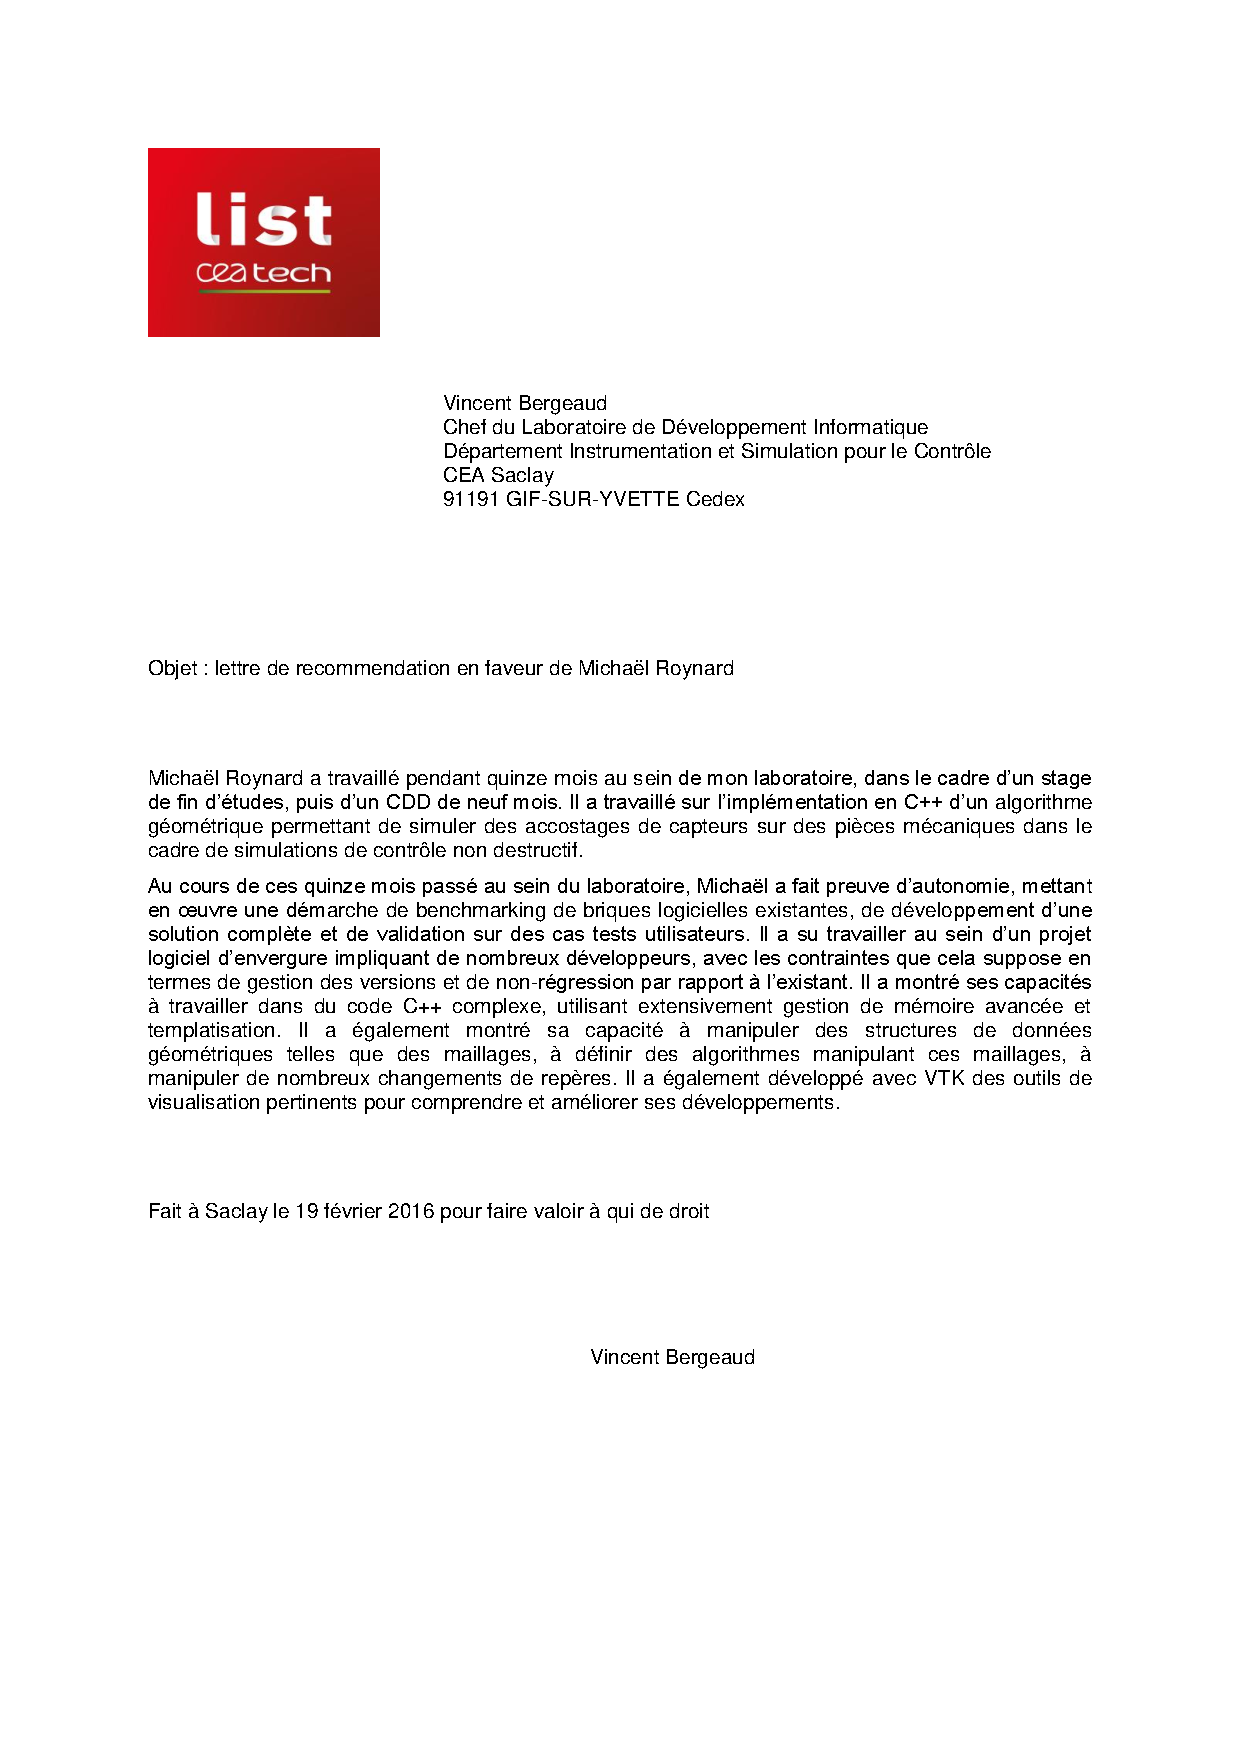
\includegraphics[scale=1.0]{lettre_recommendation_MRO.pdf}

\renewcommand{\refname}{Références bibliographiques}

\bibliographystyle{abbrv}
\bibliography{bibliography}

\end{document}